\documentclass[10pt,a4paper]{article}
\usepackage[utf8]{inputenc}
\usepackage[english]{babel}
\usepackage[T1]{fontenc}
\usepackage{amsmath}
\usepackage{amsfonts}
\usepackage{amssymb}
\usepackage{subcaption}
\usepackage{makeidx}
\usepackage{graphicx}
\usepackage{fourier}
\usepackage{listings}
\usepackage{color}
\usepackage{hyperref}
\usepackage[left=2cm,right=2cm,top=2cm,bottom=2cm]{geometry}
\author{Tommy Müller, Marcus Dittrich, Vincent Noculak}
\title{Zeeman-Effekt}

\lstset{language=C++,
	keywordstyle=\bfseries\color{blue},
	commentstyle=\itshape\color{red},
	stringstyle=\color{green},
	identifierstyle=\bfseries,
	frame=single}
\begin{document}

\maketitle
\newpage
\newpage

\section{ Theoretische Vorbereitung}

Das Rastertunnelmikroskop ist eine Vorrichtung, mit der sich Festkörperstrukturen in atomarer Größenordnung auflösen und graphisch darstellen lassen. Der Versuchsaufbau besteht prinzipiell aus einer, wenn möglich einatomigen Spitze, welche sich mittels eines piezoelektrisches Elementes über die Probenoberfläche bewegt. Der Messkopf wird dabei der Probe bis auf wenige $\AA$ angenähert, bis die Überlagerung der Wellenfunktionen von Probe und Spitze es ermöglichen, das Elektronen die Potentialbarriere zwischen beiden Materialien überwinden können und diese "durchtunneln". Der dabei messbare Tunnelstrom gibt Aufschlüsse über die lokale Zustandsdichte der Probe, aus der man Rückschlüsse auf dessen Struktur an der Oberfläche ziehen kann. \\ \\Das "durchtunneln" einer endlichen Potenzialbarriere, welche höher als die kinetische Energie des "durchtunnelnden" Teilchens ist, kann nur mit Hilfe der Quantenmechanik erklärt werden. In der quantenmechanischen Betrachtungsweise wird das Teilchen als Wellenfunktion in der Schrödingergleichung angenommen und besitzt dadurch eine gewisse Wahrscheinlichkeit die Barriere zu durchdringen. Anschaulich lässt sich dies, bei dem eindimensionalen Tunnelvorgang durch ein rechteckiges Potential der Breite d und Höhe $\Phi$ darstellen, wie in Figure 1 gezeigt.
\begin{figure}[h]
	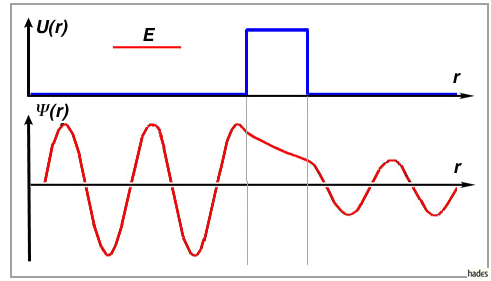
\includegraphics[scale = 0.8]{tunnel.png}
	\centering
	\caption{Abbildung Eindimensionaler Tunneleffekt}
	\label{diagramm_aufspaltung}
\end{figure}
Die Wellenfunktion des Teilchens lässt sich in drei Teile vor ($\Psi_{1}$), in ($\Psi_{2}$) und hinter ($\Psi_{3}$) der Barriere aufteilen. Eine mögliche Lösung für $\Psi$ sieht wie folgt aus:\\
$$\Psi_{1}= -\frac{k_{2}}{k_{1}}sin(k_{1}x) + cos(k_{1}x)$$ 
$$\Psi_{2}= e^{-kx}$$
$$\Psi_{3}= e^{-k_{2}d}(-\frac{k_{2}}{k_{1}}sin(k_{1}(x-d)) + cos(k_{1}(x-d)))$$
$$ k_{1} = \frac{1}{\hbar}\sqrt{2mE} $$
$$k_{2} = \frac{1}{\hbar}\sqrt{2m(E-V_{0})}$$
\\Die Amplitude der einfallenden Wellenfunktion nimmt im Bereich der Potenzialbarriere exponentiell, in Abhängigkeit von der Breite und Höhe der Barriere, ab. Somit gilt für das Teilchen hinter dem Potential eine, von d abhängige Aufenthaltswahrscheinlichkeit, für welche gilt: $\left \langle \Psi  \right \rangle^{2} > 0$. Daraus folgt, das einfallenden Teilchen eine reale Wahrscheinlichkeit besitzen, die Potenzialbarriere zu durchdringen, was zu einem messbaren Tunnelstrom führt. \\ \\Das, für die Rastertunnelmikroskopie relevante Potenzialtopf-Modell lässt sich analog zum eben beschriebenen Modell der eckigen Potenzialbarriere skizzieren. Spitze und Probe sind leitende Festkörper, deren Fermi-Niveaus sich durch eine angelegte Spannung zwischen Probe und Spitze zueinander verschieben, wodurch Elektronen in unbesetzte Niveaus der anderen Elektrode gelangen können. Die Höhe des Potentials lässt sich aus der Differenz der Elektronenaustrittsarbeiten von Probe und Spitze ermitteln.
\begin{figure}[h]
	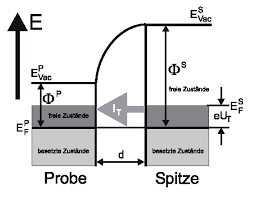
\includegraphics[scale = 1.2]{potentialtopf.png}
	\centering
	\caption{Potentialtopf-Modell zwischen Probe und Spitze}
	\label{diagramm_aufspaltung}
\end{figure} 
In Figure 2 wird dieses Konzept schematisch erfasst. Für den, sich ergebenden Tunnelstrom, lässt sich näherungsweise in Abhängigkeit vom Abstand, zwischen Probe / Spitze und der Austrittsarbeit für kleine Probenspannungen festhalten: 
\begin{equation}
I_{t} \sim V_{t} * e^{-c*\sqrt{\Phi }*d}
\end{equation}
Da man von Austrittsarbeiten in der Größenordnung mehrerer eV ausgehen kann, führt eine Änderung des Abstandes um 1 $\AA$ zu einer Variation des Tunnelstroms um etwa eine Größenordnung. Diese extreme Abstandsabhängigkeit führt dazu, das man Aussagen im Atomaren Bereich über die elektronische Struktur der Probenoberfläche treffen kann. \\ \\Für die Rastertunnelmikroskopie gibt es im allgemeinen zwei verschiedene Operationsmodi. Im ersten misst man den Tunnelstrom bei konstantem Abstand zwischen Probe und Spitze, im zweiten misst man den Abstand bei konstant gehaltenem Tunnelstrom. Dies ist der, in unserem Versuch verwendete, Operationsmodus. \\Um den Abstand zwischen Spitze und Probe so zu variieren, damit der Tunnelstrom konstant bleibt, wird im allgemeinen ein Regelkreis verwendet. Dieser wirkt der Abweichung einer physikalischen Größe über negative Rückkopplung entgegen, d.h. die Änderung einer bestimmten Größe führt zur proportionalen Änderung einer anderen Größe, welche an das Eingangssignal negativ gekoppelt ist. Vereinfacht gesagt wird der Abstand verringert / vergrößert, je nachdem, ob der gemessene Tunnelstrom größer / kleiner als der festgelegte Wert ist. Um diese Abstandsänderungen im $\AA$-Bereich vornehmen zu können, wird ein Piezoelektrisches Element verwendet. Der diesem Bauteil zugrunde liegende Piezoelektrische Effekt besagt, das eine mechanische Verformung bestimmter Festkörper, zu einer Verschiebung des Ladungsschwerpunktes innerhalb des Materials führt, wodurch elektrische Dipole entstehen, welche eine Spannung induzieren.
\begin{figure}[h]
	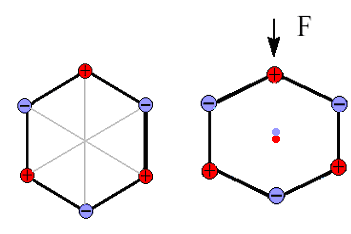
\includegraphics[scale = 1]{1piezo.png}
	\centering
	\caption{Schematische Darstellung des Piezoelektrischen Effekts}
	\label{diagramm_aufspaltung}
\end{figure}
Anschaulich lässt sich dies an Figure 3 nachvollziehen. Grundvoraussetzung ist eine symmetrische Verteilung unterschiedlich geladener Ionen im Festkörper, deren Ladungsschwerpunkte sich überlagern, wodurch, im nicht verformten Zustand, kein elektrisches Feld zustande kommt. Für ein piezoelektrisches Element wird der inverse Piezoelektrische Effekt benutzt. Dieser besagt, dass auch das anlegen einer Spannung zur mechanischen Verformung eines infrage kommenden Festkörpers führt. Somit wird die angelegte Piezospannung, für das Piezoelement in Z-Richtung, über den Regelkreis so korrigiert, damit der Tunnelstrom konstant gehalten wird. Ziel unserer Rastertunnelspektroskopie ist es, einen vorher festgelegten (X,Y) Bereich "abzurastern" um Informationen über die Elektronenzustandsdichte der Fläche zu bekommen. Um diese Bewegung im nm-Bereich zu gewährleisten, wird der Messkopf in (X,Y)-Richtung auch über ein Piezoelement manövriert. Möchte man die entstehende Realbildaufnahme untersuchen, muss man zunächst um die Struktur der, zu untersuchenden, Graphitprobe wissen.
Graphit ist neben Diamant und Fulleren die dritte unter irdischen Normalbedingungen stabile Form des Kohlenstoffes und kristallisiert meist im hexagonalen Kristallsystem.Es gehört der Mineralklasse "Elemente - Halbmetalle, Nichtmetalle" an. 
\begin{figure}[h]
	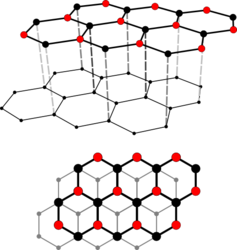
\includegraphics[scale = 1.1]{Graphit.png}
	\centering
	\caption{Aufbau des Graphits}
	\label{diagramm_aufspaltung}
\end{figure}
Wie in Figure 4 zu erkennen, besteht der ausgedehnte Kristall aus gestapelten Basalschichten A und B, die so angeordnet sind, das jeweils drei Kohlenstoffatome einer hexagonalen Zelle über drei Kohlenstoffatomen der darunterliegenden Schicht sitzen. Dies wirkt sich auf die Realbildaufnahme mit dem Rastertunnelmikroskop aus, da ein Kohlenstoffatom der Basalschicht B, welches senkrecht unter einem Atom der Schicht A liegt, dessen elektronische Struktur so beeinflusst, das die gemessene Elektronenzustandsdichte wesentlich geringer ist, als bei den, in Figure 4 rot markierten, Kohlenstoffatomen. Dies führt dazu, das wir in der Aufnahme der atomaren Struktur eben diese Atome sehen, wodurch der Eindruck eines größeren Abstandes zwischen den angeordneten Atomen entstehen kann. Eine weitere wichtige Eigenschaft des Graphits ist es, das die Bindungsenergie innerhalb einer Schicht deutlich größer ist, als die Bindungsenergie zwischen den Schichten (4.3eV zu 0.07eV). Dies führt dazu, das es leichter ist eine Schicht vom Kristall zu lösen, als einzelne Atome aus einer Schicht. Deswegen ist es uns möglich, Stufenkanten und Plateaus am Graphit zu untersuchen, da diese größtenteils erhalten bleiben. Des weiteren führt dies zu einer fast metallischen Leitfähigkeit entlang einer Ebene. Wichtige Kenngrößen sind außerdem der Abstand zwischen zwei Kohlenstoffatome in einer Schicht und der Abstand zwischen zwei übereinander liegenden Kohlenstoffatomen:
$$a = 2.46 \AA$$
$$c = 6.71 \AA$$
Um weitere Informationen und Schlussfolgerungen aus den ermittelten Bildern zu ziehen, unterzieht man die aufgenommenen Topographien einer zweidimensionalen Fouriertransformation. Dabei werden die Bilder vom Real in den Impulsraum, den sogenannten Reziproken Raum, abgebildet, wodurch periodische Strukturen besser zu erkennen sind. Durch Rücktransformation lassen sich verzerrende Wellenfunktionen extrahieren und man bekommt eine schärfere Abbildung im Realraum.
  

\section{	Versuchsaufbau}

Das, in unserem Versuch verwendete Raster-Tunnelmikroskop ist ein Eigenbau der Arbeitsgruppe und arbeitet unter atmosphärischem Druck. Die Bewegung des Messkopfes in X-Y-Z-Richtung wird über einen PC mit der Freeware WSxM der Firma Nanotec gesteuert.  Der schematische Aufbau lässt sich anhand von Figure 5 nachvollziehen.  Die Z-Richtung des Messkopfes wird über einen Regelkreis variiert, um den Tunnelstrom konstant zu halten. Die Bewegung des (X,Y)-Piezo wird über einen Scangenerator gesteuert. Die ankommenden Signale werden verstärkt und an den Messkopf und Spitze weitergeleitet um diese zu bewegen.  Dieser Messkopf besteht im Wesentlichen aus einem Piezo-Röhren-Scanner und einer Messspitze aus einer Titan-Iridium Legierung. Der gemessene Tunnelstrom wird durch einen Strom- / Spannungswandler geschickt, um die gemessenen Ströme (1nA) als Spannung im mV-Bereich besser auswerten zu können. Anschließend werden die Daten logarithmiert um einen größeren Messumfang ohne Bereichsumschaltung zu erreichen. Das Ausgangssignal wird dann an die Bilderzeugung und an den Regler weitergeleitet und der Kreislauf beginnt von neuem. Der gesamte Versuchsaufbau wurde auf einem schwingungsgedämpften Tisch installiert, um Messfehler durch Vibrationen zu minimieren. Des weiteren befindet sich über dem Versuchsaufbau eine Schutzglocke, um den Messaufbau vor Luftströmen und weiteren Verunreinigungen zu bewahren.

\begin{figure}[h]
	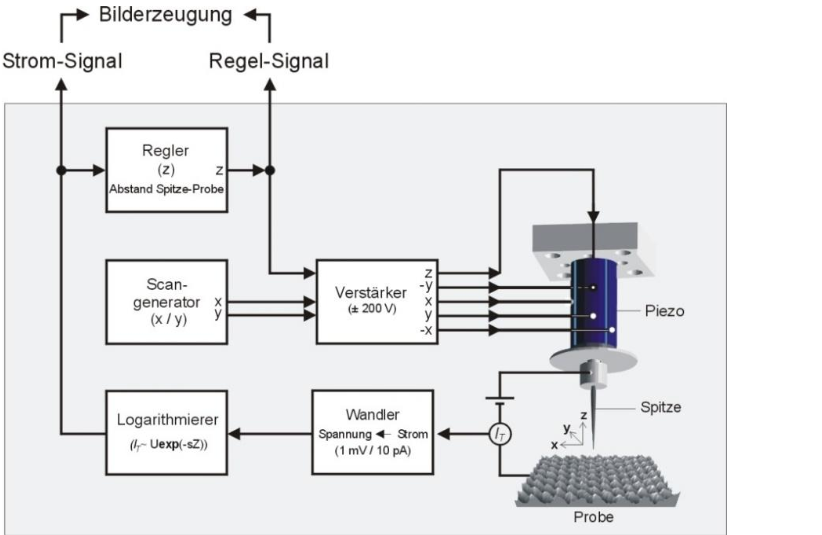
\includegraphics[scale = 0.6]{aufbau.png}
	\centering
	\caption{Blockschaltbild eines Rastertunnelmikroskops}
	\label{diagramm_aufspaltung}
\end{figure}

\section{Durchführung}

Bevor Messungen am Versuchsaufbau durchgeführt werden können, müssen Messspitze und Graphitoberfläche präpariert werden. Dafür wurde die alte Messspitze zunächst aus dem Aufbau entfernt und mit einer Zange so abgekniffen, dass eine möglichst dünne Spitze erzeugt wurde. Des Weiteren wurde mit einer Lage Tesafilm die oberste Schicht der Graphitprobe entfernt, um mögliche Verunreinigungen zu entfernen und Stufenkanten, bzw. Plateaus zu generieren. Anschließend haben wir die Spitze wieder in den Messkopf eingesetzt und mittels einer Mikrometerschraube per Hand an die Probe angenähert. Mit Hilfe eines Schrittmotors wurde die Spitze dann bis auf wenige $\AA$ angenähert, bis ein vorher festgelegter Tunnelstrom messbar war. Danach wurde der Motor abgenommen und die Schutzglocke aufgesetzt. Anschließend haben wir verschiedene Messungen mit Variationen der Parameter, wie z.B. der angelegten Bias Spannung (zwischen Probe und Spitze) oder des festgelegten Tunnelstroms durchgeführt, um möglichst gute Aufnahmen der Graphit-Oberfläche zu bekommen. Atomare Auflösung konnten wir dabei allerdings nicht erreichen.

\subsection{Parameter}

Zunächst wurde der Messaufbau, wie in der Durchführung beschrieben hergerichtet. Wichtige Parameter sind Size, Speed, Bias, Set Point, Z Gain und der Logarithmic Feedback. Size bestimmt die Kantenlänge der untersuchten Probenoberfläche in nm und der Parameter Speed gibt die Scangeschwindigkeit einer Linie in s an. Bias beschreibt die angelegte Probenspannung in mV und Set Point charakterisiert den konstanten Tunnelstrom während der Messung. Der Z-Gain ist die eingestellte Hochspannungsverstärkung für die Z-Bewegung. Die Funktion des Logarithmic Feedbacks besteht darin, den Fehler zwischen dem gewünschten Sollwert und den Gemessenen Werten zu berechnen. 

$$u(t) = K_{p}e(t)+K_{i}  \int_{0}^{t}e(\tau)d\tau$$

Der Proportionale Term erzeugt einen Ausgangswert, der proportional zum Fehlerwert ist und der Integral Term summiert die momentanen Fehler über einen Zeitbereich. Ein kleiner Proportional Gain führt bei einem kleinen Ausgabewert zu einem großen Eingangsfehler.  Sind Proportional und Integral Gain zu hoch, wird der Fehler nicht stabil. In Table 1 haben wir unsere, während der Messung verwendeten, Parameter aufgelistet.

\begin{table}[]
	\centering
	\caption{Messparameter}
	\label{Messparameter}
	\begin{tabular}{ll}
		Size (nm)           & 3-30      \\
		Speed (lines / sec) & 1.831     \\
		Points              & 256       \\
		Bias (mV)           & 1000      \\
		Set Point (nA)      & 1-30      \\
		Signal Gain         & 1         \\
		Z Gain              & 1         \\
		Proportional Gain   & 0.2 - 1.8 \\
		Integral gain       & 0.1 - 0.9
	\end{tabular}
\end{table}



\section{Quellen}
(Figure 1):\url{https://elearning.physik.uni-frankfurt.de/data/FB13-PhysikOnline/lm_data/lm_282/auto/kap26/picts/tunnel.gif}\\
(Figure 2):\url{http://www.uni-ulm.de/physchem-praktikum/media/fp/v_11.pdf}\\
(Figure 3):\url{http://www.piezoeffekt.de/bilder/1piezo.gif}\\
(Figure 4): \url{https://upload.wikimedia.org/wikipedia/commons/thumb/5/54/GraphitGitter4.png/237px-GraphitGitter4.png}\\
(Figure 5): Blockschaltbild eines Raster-Tunnelmikroskops von Frank Trixler, Ludwig-Maximilians-Universität München (Aus der Anleitung)
\end{document}